% Template for the submittion to:
%   The Annals of Probability           [aop]
%   The Annals of Applied Probability   [aap]
%   The Annals of Statistics            [aos]
%
%Author: In this template, the places where you need to add information
%        (or delete line) are indicated by {???}.  Mostly the information
%        required is obvious, but some explanations are given in lines starting
%Author:
%All other lines should be ignored.  After editing, there should be
%no instances of ??? after this line.

% use option [preprint] to remove info line at bottom
% journal options: aop,aap,aos
%\documentclass[aos]{imsart}
\documentclass{imsart}

\usepackage{amsthm,amsmath,natbib}
%\RequirePackage[dvips]{hyperref}

% use this package if hyperref and natbib is used:
%\RequirePackage{hypernat}

% provide arXiv number if available:
%\arxiv{math.PR/0000000}

% put your definitions there:
\startlocaldefs

\usepackage{graphics,amssymb,color}
\usepackage{graphicx,subfigure}
\usepackage[boxed]{algorithm2e}

\newcommand{\argmax}{\mathop{\mathrm{argmax}}}
\newcommand{\argmin}{\mathop{\mathrm{argmin}}}
\newcommand{\minimize}{\mathop{\mathrm{minimize}}}
\newcommand{\maximize}{\mathop{\mathrm{maximize}}}

\newcommand{\todo}{\textcolor{red}{\textbf{To do: }}}

\newcommand{\real}{\mathbb{R}}
\newcommand{\Pp}{{\mathbb P}}
\newcommand{\Ee}{{\mathbb E}}
\newcommand{\lips}{{\cal L}}
\newcommand{\tube}{\mathrm{Tube}}
\newcommand{\sphere}[1]{O^{#1-1}}
\newcommand{\dimens}{\text{dim}}
\newcommand{\cone}{\text{Cone}}
\newtheorem{theorem}{Theorem}
\newtheorem{lemma}[theorem]{Lemma}
\newtheorem{cor}[theorem]{Corollary}
\newcommand{\XK}{K_X}
\newcommand{\norm}[1]{\lVert #1 \rVert}
\newcommand{\innerp}[2]{\langle #1 , #2 \rangle}
%\newcommand{\qed}{\hfill $\Box$\newline}

\newcommand{\grad}{\nabla}
\newcommand{\V}{\mathcal{V}}\endlocaldefs
\newcommand{\K}{\mathcal{K}}
\newcommand\tf{\widetilde{f}}
\newcommand{\pen}{\mathcal{P}}

\begin{document}

\begin{frontmatter}

% "Title of the paper"
\title{A significance test in forward stepwise model selection}

%%%
%%% \runtitle{} - I don't know what this is
%%%

% indicate corresponding author with \corref{}
\author{\fnms{Jonathan} \snm{Taylor}\corref{Jonathan E. Taylor}\ead[label=e1]{jonathan.taylor@stanford.edu}\thanksref{t1}
\and \fnms{Joshua} \snm{Loftus}
\and ???}
\thankstext{t1}{Supported in part by NSF grant DMS 1208857 and
AFOSR grant 113039.}

\affiliation{Stanford University}

\address{Department of Statistics\\  Stanford University\\ Sequoia
Hall \\390 Serra Mall\\ Stanford, CA 94305, U.S.A.\\ \printead{e1}}

%%%
%%% \runauthor{Taylor} - I don't know what this is
%%%

\begin{abstract}
% perhaps de-emphasize group lasso and emphasize forward stepwise?
  We apply the methods of \cite{tests:adaptive} and
  \cite{significance:lasso} on significance tests for penalized
  regression to forward stepwise model selection. For the $k$th
  variable to enter the model, previous work relied on an asymptotic
  null distribution that breaks down when grouped variables are
  entering the model and is difficult to derive. We iteratively apply
  an exact null distribution for the first (potentially grouped)
  variable on the residual from previous steps. The resulting method
  has the strengths of stepwise selection, for example parallel
  computation, but also remedies the problem of inflated test
  statistics and over-fitting.
\end{abstract}

%%%
%%% - Gotta change these
%%%
\begin{keyword}[class=AMS]
\kwd[Primary ]{62M40}
%\kwd{}
\kwd[; secondary ]{62H35}
\end{keyword}

\begin{keyword}
\kwd{penalized regression}
\kwd{convex analysis}
\kwd{least squares}
\kwd{Gaussian processes}
%\kwd{extreme value theory}
\end{keyword}

\end{frontmatter}


\section{Introduction}
\label{sec:intro}

Forward stepwise regression is a stochastic model selection procedure
that begins with an empty model and adds the best predictor variable
in each step.  Classical significance tests fail when a model has been
selected this way and tend to be anti-conservative.  Recently,
\cite{significance:lasso} found a novel test statistic with an
appropriate null distribution that behaves well when a model has been
selected using the lasso \citep{tibshirani:lasso}.
\cite{tests:adaptive} modified and extended those results to the
group lasso \citep{grouplasso} and other adaptive regression
problems.  The present work explores the behavior of those test
statistics for models selected by forward stepwise procedures and
works out some of the details involved in applying these methods to
models with grouped variables.  Our test statistic can be
used for valid significance testing when computed from the same
data as the model selection.  The resulting method can
be more statistically efficient than validation on held-out data, and
also more computationally efficient than penalized methods with
regularization parameters chosen by cross-validation.



(\todo Change this paragraph as the sections are completed)
In Section \ref{sec:stepwise} we establish notation and describe our
forward stepwise procedure. Section \ref{sec:testing} briefly reviews
the parts of \cite{significance:lasso} and \cite{tests:adaptive}
relevant to our significance test, and describes the group lasso which
we require for applying the test with grouped
variables. Simulation results in Section \ref{sec:simulations} using
various stopping rules for the forward stepwise procedure--including
some from \cite{sequential:fdr}--appear promising.

%%%%%%%%%%%%%%%%%%%%%%%%%%%%%%%%%%%%%%%%%%%%%%%%%%%%
%%%%%%%%%%%%%%%%%%%%%%%%%%%%%%%%%%%%%%%%%%%%%%%%%%%%
%%%%%%%%%%%%%%%%%%%%%%%%%%%%%%%%%%%%%%%%%%%%%%%%%%%%

\section{Forward stepwise model selection}
\label{sec:stepwise}

We allow forward stepwise selection to add groups of variables in each
step, not only in the case of binary encoding for categorical
variables but also for any grouping purpose. For example, groups of
variables may be pre-designated factors such as expression
measurements for all genes in a single functional pathway. An entire
group is included or excluded together from the final model. For
consistency we will use $g, h$ as indices rather than the usual $i, j$
throughout. Since single variables can be considered groups of size 1,
our general exposition includes non-grouped situations as a special case. 

Label the outcome variable of $n$ i.i.d. measurements $y \in \real^n$. Let an integer $G \geq 1$ 
be the number of groups. For each $1 \leq g \leq G$ the design matrix encoding the
$g$th group is the $n \times p_g$ matrix denoted $X_g$, where $p_g$ is
the number of individual variables in group $g$. Define $p = \sum_{g=1}^G
p_g$ the total number of individual variables, so $p = G$ in the
case where all groups have size 1. Let $X$ be the matrix constructed
by column-binding the $X_g$, that is  
%Throughout most of this paper we assume orthogonality within groups, that is
%$X_g^T X_g = I_{p_g \times p_g}$ for all $g$. ( \todo Take this out if
%we don't actually need it).  
%%%%%%%%%%%%%%%%%%%%%%%%%%%%%%%%%%%%%%%%%%%%%%%%
\begin{equation*}
X = \begin{pmatrix} X_1 & X_2 & \cdots & X_G  \end{pmatrix}
\end{equation*}
%%%%%%%%%%%%%%%%%%%%%%%%%%%%%%%%%%%%%%%%%%%%%%%%
With each group we associate the $p_g \times 1$ coefficient vector
$\beta_g$, and write $\beta$ for the $p \times 1$ vector constructed
by stacking all of the $\beta_g$ in order.  Finally, our model for the
response is
%%%%%%%%%%%%%%%%%%%%%%%%%%%%%%%%%%%%%%%%%%%%%%%%
\begin{equation}
\begin{aligned}
\label{eq:gmodel}
y & = X \beta + \sigma \epsilon \\
   & = \sum_{g=1}^G X_g \beta_g + \sigma \epsilon
\end{aligned}
\end{equation}
%%%%%%%%%%%%%%%%%%%%%%%%%%%%%%%%%%%%%%%%%%%%%%%%
where $\epsilon$ is noise. Unless otherwise specified we assume
i.i.d. Gaussian noise $\epsilon \sim N(0, I_{n \times n})$ and that
$\sigma$ is known.

We allow for the possibility $p > n$ in which case \ref{eq:gmodel} is
generically underdetermined. In such cases it still may be possible to
estimate $\beta$ well if it is sparse--that is, if it has few nonzero
entries \citep{donoho:pursuit}. In the rest of this paper we refer to
variable groups $X_g$ as noise variables if $\beta_g$ is a zero vector
and as true predictor variables if $\beta_g$ has nonzero entries.

Before we describe the forward stepwise procedure we require one last
ingredient. To each group of variables we assign a weight $w_g$. These
weights act like penalties or costs, so increasing $w_g$ makes it
more difficult for the group $X_g$ to enter the model. The
modeler can choose weights arbitrarily, but we will only use one
particular choice, based on $p_g$, that we discuss later. With this we
are ready to describe the forward stepwise procedure, given in Algorithm
\ref{algo:fs}. Note that to enable our p-value computations,
\textit{max.steps} should be at most $\min (n, G) - 1$. In our
implementation we treat the active set $A$ as an ordered set to easily
track the order of variables entering the model.

\begin{algorithm}
\DontPrintSemicolon
\KwData{An $n$ vector $y$ and $n \times p$ matrix $X$ of $G$ grouped variables}
\KwResult{Active set $A$ of variable groups included in the model}
\SetKwFunction{lsfitResidual}{lsfitResidual}
\caption{Forward stepwise procedure with groups and weights}
\BlankLine
$A \gets \emptyset$\;
$A^c \gets \{ 1, \ldots, G \}$\;
$r_0 \gets y$\;
\For{$step \leftarrow 1$ \KwTo $max.steps$}{
  $g^* \gets \argmax_{g \in A^c} \norm{X_g^T r_{g-1}}_2 / w_g$\;
  $A \gets A \cup \{ g^* \}$\;
  $A^c \gets A^c \backslash \{ g^* \}$\;
  \For{$g \in A^c$}{
    $X_g \gets (I - X_{g^*}X_{g^*}^\dagger) X_g$;
  }
  $r_g \gets $\lsfitResidual{$r_{g-1}, X_{g^*}$}\;
}
\KwRet{$A$}
\label{algo:fs}
\end{algorithm}


Subset selection refers to the problem of choosing a subset of the $p$
potential variables to include in a model. Since there are $2^p$ such
choices, exhaustive search is computationally infeasible when $p$ is
large. If exhaustive search were possible, performing a large
search runs the risk of over-fitting unless model complexity is
appropriately penalized. Algorithm \ref{algo:fs} produces a much
smaller set of potential models, at most \textit{max.steps}. However,
it is a greedy algorithm so the set of models it produces may not
contain the best possible model. This is an inherent shortcoming which
we do not address in this paper.

So far we have left open the question of choosing among the models in
the forward stepwise sequence, i.e. when to stop stepping
forward. Some classical approaches can be posed as optimization
criteria which stop at the step minimizing
\begin{equation}
\begin{aligned}
\label{eq:subsetregress}
\frac{1}{2} \| y - X \beta_s \|_2^2 + \lambda \pen(\beta_s)
\end{aligned}
\end{equation}
where we have written $\{ \beta_s : s = 1, \ldots, max.steps \}$ as
the sequence of models outputted by forward stepwise. The function
$\pen(\beta)$ is a penalty on model complexity usually taken to be the
number of nonzero entries of $\beta$. Proposals for $\lambda$ include
2 ($C_p$ of \cite{CP}, AIC of \cite{AIC}), $\log(n)$ (BIC of \cite{BIC}), and
$2\log(p)$ (RIC of \cite{RIC}). In the current paper we provide
accurate p-values when adding the first noise variable group in the forward
stepwise sequence, and it is natural to consider using these p-values
to choose a model. \cite{sequential:fdr} examined some stopping rules
using the asymptotic p-values of \cite{significance:lasso} and showed
their stopping rules control false discovery rate--the expected
proportion of noise variables among variables declared significant
\citep{fdr}. We explore this further in Section \ref{sec:simulations}.

Although forward stepwise is a greedy algorithm producing a
potentially sub-optimal sequence of models, under favorable conditions
it can still perform well. There is a parallel literature to the
compressed sensing literature \textit{(cite some here)} with theorems
stating that forward stepwise can exactly select the true model under
some stringent conditions involving quantities like the sparsity of
the true model and the coherence of the design matrix. We do not
pursue this any further because we find empirically that forward
stepwise can work well in much less restrictive situations than those
guaranteed by theorems.

To explore the performance of forward stepwise empirically we
conducted simulations with results shown in ~\ref{fig:fwdstepsims}


\begin{figure}
\begin{center}
\subfigure[Gaussian design]{
%\label{fig:smallgauss}
\includegraphics[width=0.5\textwidth]{../figs/fwdstep/gaussian_p2n_n100_lower1p4_upper1p6.pdf}}
\hspace{-15pt}
\subfigure[Categorical design]{
%\label{fig:smallcat}
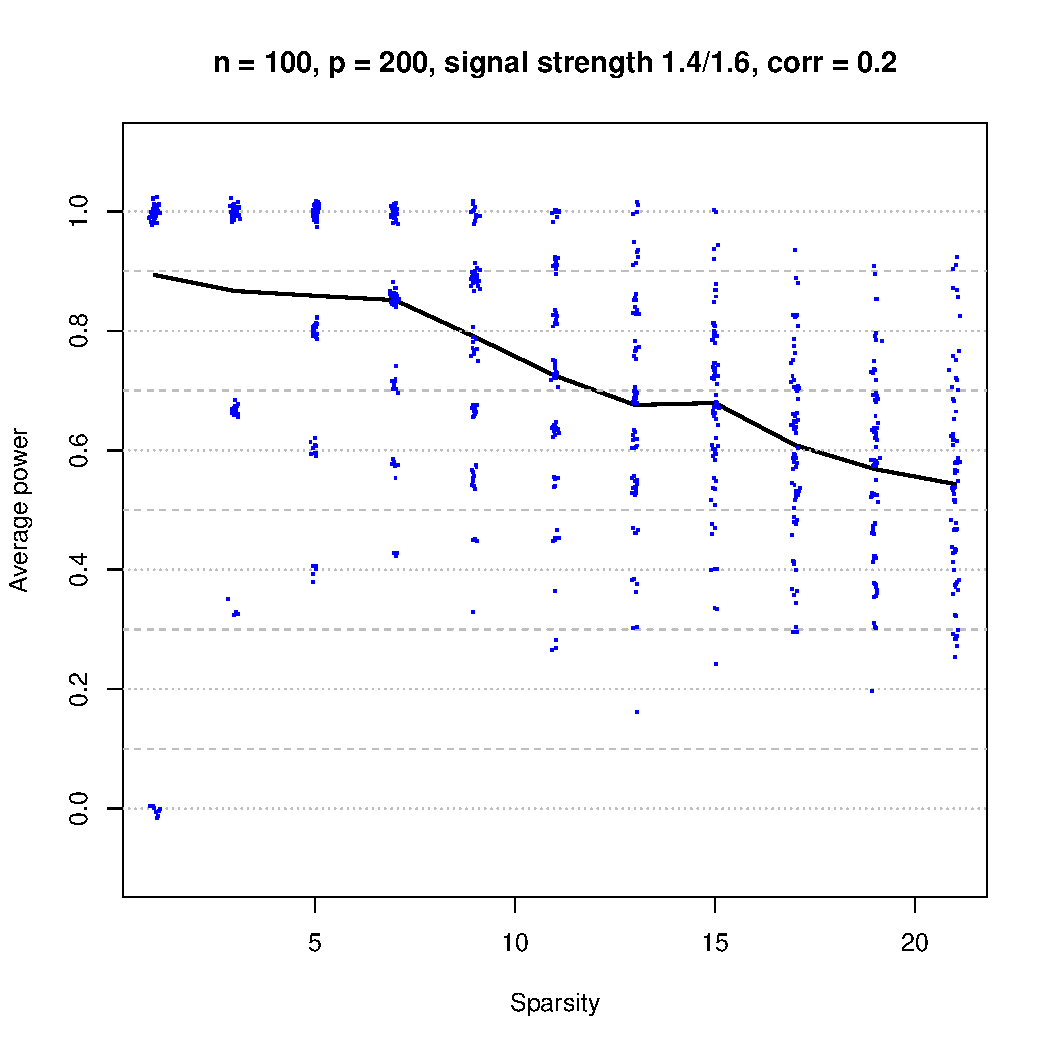
\includegraphics[width=0.5\textwidth]{../figs/fwdstep/gaussian_p2n_n100_lower1p4_upper1p6_corr0p2.pdf}}
\caption{\small \it The left panel shows results of a simulation with
  an independent Gaussian design matrix and a signal vector having
  three groups with non-zero coefficients of sizes one, two, and
  three, and seven groups of noise variables with sizes varying from
  one to ten, for a total of 30 variables. For the right panel we
  repeated this setup, but group sizes corresponded to levels of
  categorical variables. The groups of size one were increased to two,
so there are 10 categorical variables with a total of 32 levels.}
\label{fig:fwdstepsim}
\end{center}
\end{figure}




%%%%%%%%%%%%%%%%%%%%%%%%%
%%%%%%%%%%%%%%%%%%%%%%%%%

\section{Significance testing: from lasso to group lasso}
\label{sec:testing}

\todo Update this section to match/complement \citep{tests:adaptive}



In the ordinary least squares setting, a significance test for a
single variable can be conducted by comparing the drop in residual
sums of squares (RSS) to a $\chi^2_1$ distribution. Similarly, when
adding a group of $k$ variables we can compare the drop in RSS to a
$\chi^2_k$ random variable. This generally does not work when the
variable to be added has been chosen by a method that uses the data,
and in particular it fails for forward stepwise procedures adding
the ``best'' (e.g. most highly correlated) predictor in each step. In
that case, the test statistic (drop in RSS) does not match the
theoretical null distribution even when the null hypothesis is
true. \cite{significance:lasso} introduced a new test statistic based
on the knots in the lasso solution path. They derived a simple
asymptotic null distribution, proved a type of convergence under broad
``minimum growth'' conditions, and demonstrated in simulations that
the test statistic closely matches its asymptotic distribution even in
finite samples.  That work marked an important advance in the problem
of combining inference with model selection.  The current paper
extends some of their results to the group lasso \citep{grouplasso}.
In the process we had to derive an exact finite sample null
distribution for the test statistic, this appears in
\cite{tests:adaptive}. 


Writing $\hat \beta(\lambda)$ for the lasso solution for a fixed value of $\lambda$, we need
the following facts summarized in \cite{significance:lasso} (ref Tibs2012?).

\begin{itemize}

  \item The vector valued function $\hat \beta(\lambda)$ is a
    continuous function of $\lambda$. For the lasso path, the
    coordinates of $\hat \beta(\lambda)$ are piecewise linear with
    changes in slope occurring at a finite number of $\lambda$ values
    referred to as \emph{knots}. The knots depend on the data and are
    usually written in order $\lambda_1 \geq \lambda_2 \geq \cdots
    \geq \lambda_r \geq 0$. We follow this convention. 

  \item The \emph{active set} $A_k$ is a set of indices of variables
    for which the corresponding coordinates of $\hat \beta(\lambda_k)$
    are potentially nonzero. Any variable with index not in $A_k$ has
    a zero coefficient in $\hat \beta(\lambda_k)$, but the converse is
    not true. \todo{is this equicorrelation set?}
  
  \item Path algorithms for computing lasso solutions proceed by
    fitting models at a grid of $\lambda$ values. The active set
    changes whenever $\lambda$ crosses a knot, and predictor variables
    can both enter and leave the active set. However, at the first two
    knots $\lambda_1$ and $\lambda_2$ no variable can leave the active
    set. So the first two knots correspond to the first two variables
    entering the model. 

\end{itemize}

\cite{significance:lasso} prove that under the null hypothesis that $A_k$
contains all the strong predictor variables, the distribution of a
test statistic $T_k \propto \lambda_k(\lambda_k - \lambda_{k+1})$ is
asymptotically Exp(1). In the lasso case we know a lot about the knots
and active set, but the group lasso picture is slightly more
complicated. For the group lasso, $\hat \beta(\lambda)$ does not have
piecewise linear components. To overcome this difficulty we will
restrict our attention to the first group of variables to enter the
active set since the analysis then follows almost exactly as for the
lasso. (\todo Change this if I can find $\lambda_k$). 

The \emph{group lasso estimator} is the following solution to a convex
problem
%%%%%%%%%%%%%%%%%%%%%%%%%%%%%%%%%%%%%%%%%%%%%%%%
\begin{equation}
\begin{aligned}
\label{eq:gsoln}
\displaystyle \hat \beta_\lambda = \argmin_{\beta \in \real^p} \frac{1}{2} \| y - X \beta \|_2^2 +
   \lambda \sum_{g=1}^G w_g \| \beta_g \|_2
\end{aligned}
\end{equation}
%%%%%%%%%%%%%%%%%%%%%%%%%%%%%%%%%%%%%%%%%%%%%%%%
The parameter $\lambda \geq 0$ enforces sparsity in groups: for large
$\lambda$ most of the $\beta_g$ will be zero vectors. The weights
$w_g$ are usually taken to be $\sqrt p_g$ to normalize the penalty
across groups.  Note that this includes the usual lasso estimator as a
special case when all of the groups are of size 1, since then the
penalty term is the $L^1$-norm of $\beta$. 

%%%%%%%%%%%%%%%%%%%%%%%%%%%%%%%%%%%%%%%%%%%%%%%%
%%%%%%%%%%%%%%%% Related works %%%%%%%%%%%%%%%%%
%%%%%%%%%%%%%%%%%%%%%%%%%%%%%%%%%%%%%%%%%%%%%%%%

\todo Fix references below

The group lasso estimator is discussed in (ref that guy's thesis) and
(ref Yuan and Lin).  An important extension is the sparse group lasso
(ref ???) which enforces sparsity in groups as well as sparsity of the
coefficients within the groups.  For a survey on group lasso and
related factor models see (ref???). \todo review some more literature
and add a few more references here if they seem worthwhile. 


Before considering the group lasso, we review some ingredients of the
proof for the lasso. Let $J = \{ 1, 2, \ldots, p \}$ index variables
and consider a stochastic process $f_{j,s} = sX_j^Ty$ defined on $T =
J \times [ -1, 1 ]$. This stochastic process is simply a collection of
linear combinations of $y$, hence it is Gaussian under the assumption
of Gaussian errors. The \emph{Karush-Kuhn-Tuckher (KKT) conditions}
(ref???) imply that $\lambda_1 = \max_j |X_j^Ty|$. By introducing the
sign variable $s$, we can remove the absolute value and write
$\lambda_1$ as the maximum of our Gaussian process 

\begin{equation}
\lambda_1 = \max_{(j,s)} f_{j,s}
\end{equation}

We have exhibited the first knot as the maximum of a Gaussian
process. We can do this for the second knot by introducing a new
process. Let $(j_1, s_1)$ be the maximizer so that $\lambda_1 =
s_1X_{j_1}^Ty$, and define 
%%%%%%%%%%%%%%%%%%%%%%%%%%%%%%%%%%%%%%%%%%%%%%%%
\begin{equation}
\begin{aligned}
  f^{(j_1,s_1)}_{(j,s)} & = \frac{ sX_j^T y - s X_j^T X_{j_1} X_{j_1}^Ty  } { 1 -  ss_1 X_j^TX_{j_1}} \\
  & = \frac{ sX_j^T(I-P_{j_1}) y }{ 1 -  s_1 X_{j_1}^T X_js}
\end{aligned}
\end{equation}
%%%%%%%%%%%%%%%%%%%%%%%%%%%%%%%%%%%%%%%%%%%%%%%%
where $P_j$ is the projection onto the subspace spanned by $X_j$. We
can think of this as a ``residual process'' after regressing out the
maximum. Write $M = \max_{j \neq j_1, s} f^{(j_1,s_1)}_{(j,s)}$, the
maximum of this residual process. It can be shown from the KKT
conditions that $M  = \lambda_2$. To summarize, we have represented
the first two knots of the lasso solution path as the maxima of some
natural Gaussian processes. Distributional facts about Gaussian
processes now allow us to make conclusions about the distribution of
functions of the knots. 

\subsection{Group lasso}
To extend this argument to the group lasso we need to define Gaussian
processes that characterize the knots of the group lasso solution
path.  

\todo Either use the simplified argument in the case of equal weights
(equal group sizes), or finish adjusting the proof of $M = \lambda_2$
to include the weights and use that version. The proof can go in an
appendix. 

\todo Modify write-up to match notation with \cite{tests:adaptive} and
then paste it in here

\subsection{Better p-values}

Maybe just reference \cite{tests:adaptive}? It might be worthwhile to
leave in the connection with \cite{significance:lasso} (getting our
test statistic by not using the approximation)

\begin{itemize}

\item \todo Add the figures to this section
\item \todo Convert to exposition instead of bulleted list
\item \todo Update to reflect latest work
  \item As in LTTT, $T = \lambda_1 (\lambda_1 - M)$ and $M = \lambda_2$
  \item Convergence to the limiting Exp(1) distribution is too slow
    \[
      \frac{P(\chi_k / w_g \geq m + t/m)}{P(\chi_k / w_g \geq m)} \to e^{-t} \text{ as } m \to \infty
    \]
    (when the group achieving $\lambda_1$ is group $g$ and has rank $k$)
  \item The limiting distribution only depends on $T$, but we also observe $M$
  \item Let's just try the ratio (conditional $\chi_k$ tail probability) evaluated at $T$ and $M$ (it works better)
  \item Going one step further, instead of using the approximation (see LTTT Proof of Lemma 5)
    \[
      \frac{M + \sqrt{M^2+4t}}{2} \approx M + \frac{t}{M}
    \]
    we can just use the left hand side
  \item For $T = \lambda_1(\lambda_1 - M)$ the left hand side simplifies to $\lambda_1$
  \item Now our p-value is
    \[
      \frac{P(\chi_k / w_g \geq \lambda_1)}{P(\chi_k / w_g \geq \lambda_2)}
    \]   
\end{itemize}



\section{Simulations}
\label{sec:simulations}

\todo Expand, include simulation results (copy latex for
includegraphics etc), do the simulation comparing stopping rules

\begin{itemize}
  \item Show null and non-null p-value-by-step plots for several examples
  \item Discuss one of these carefully (perhaps with a noise variable
    entering before a signal variable), for several fixed stopping points
  \item Compare a few stopping rules, e.g. naive one(s),
    TailStop/HybridStop, AIC/BIC/Cp
  \item (the stopping comparisons are not done yet, but I am guessing
    they will be comparable, perhaps AIC/BIC/Cp will be better, and in
    that case look for other advantages of ours to mention,
    e.g. interpretability for being based on p-values rather than a
    complexity penalty)

\end{itemize}


\begin{figure}
\begin{center}
\subfigure[Gaussian design]{
\label{fig:smallgauss}
\includegraphics[width=0.5\textwidth]{../figs/gaussian_size1_n100_p200_g200_k10_lower1p8_upper1p9.pdf}}
\hspace{-15pt}
\subfigure[Categorical design]{
\label{fig:smallcat}
\includegraphics[width=0.5\textwidth]{../figs/gaussian_size1_n100_p200_g200_k10_lower1p8_upper1p9_corr0p1.pdf}}
\caption{\small \it The left panel shows results of a simulation with
  an independent Gaussian design matrix and a signal vector having
  three groups with non-zero coefficients of sizes one, two, and
  three, and seven groups of noise variables with sizes varying from
  one to ten, for a total of 30 variables. For the right panel we
  repeated this setup, but group sizes corresponded to levels of
  categorical variables. The groups of size one were increased to two,
so there are 10 categorical variables with a total of 32 levels.}
\end{center}
\end{figure}



\input{../small_sim_selection.tex}

\input{../small_sim_estimation.tex}

\begin{figure}
\begin{center}
\subfigure[Large Gaussian lasso]{
\label{fig:largelasso}
\includegraphics[width=0.5\textwidth]{../figs/gaussian_size5-10_n100_p200_g35_k10_lower1p8_upper1p9.pdf}}
\hspace{-15pt}
\subfigure[Large Gaussian group lasso]{
\label{fig:largegrplasso}
\includegraphics[width=0.5\textwidth]{../figs/gaussian_size5-10_n100_p200_g35_k10_lower1p8_upper1p9_corr0p1.pdf}}
\caption{\small \it The left panel shows results of a simulation with
  an independent Gaussian design matrix and a signal vector having
  three groups with non-zero coefficients of sizes one, two, and
  three, and seven groups of noise variables with sizes varying from
  one to ten, for a total of 30 variables. For the right panel we
  repeated this setup, but group sizes corresponded to levels of
  categorical variables. The groups of size one were increased to two,
so there are 10 categorical variables with a total of 32 levels.}
\end{center}
\end{figure}

\input{../large_sim_selection.tex}

The large simulation has 50 groups, 25 of size 1, 10 of size 5, 10 of
size 10, and 5 of size 15. Signal vectors were supported on random
choices of 10 of these groups (changing in each realization), with
non-zero signal magnitude around $\sqrt{2\log p}$ where $p = 250$
(roughly 3.3). The design matrix had 200 rows and the simulation
performed 100 realizations.



\section{Real data example}
\todo Simulation with non-Gaussian design matrix (from AIDS data probably)



\section{Discussion}
\label{sec:discuss}

\todo After finising everything else, move some points of discussion
here, re-read and see if there's anything else interesting to comment
on here. Mention ongoing work



%%%%%%%%%%%%%%%%%%%%%%%%%
%%%%%%%%%%%%%%%%%%%%%%%%%
%% Check below for latex examples if necessary %
%%%%%%%%%%%%%%%%%%%%%%%%%
%%%%%%%%%%%%%%%%%%%%%%%%%
%
%
%In the classical setting $n > p$ the system eqref{eq:LS:KKT} often has a unique solution, the familiar
%$$
%\hat{\beta} = (X^TX)^{-1}(X^Ty).
%$$
%In many parametric models, the least squares model is of course too simple. In the exponential family setting  \citep{amari,efron}, the normal equations are similar, with  $(X^TX)$ replaced  by the observed Fisher information. We have focused on squared error-loss
%for its simplicity of exposition.
%
%In high-dimensional settings, $n$ is often less than $p$ and there is of course no unique solution 
%to eqref{eq:LS:KKT}. Many modifications are possible, for instance ridge or Tikhonov regularization which adds a strongly convex quadratic term to . The addition of such quadratic terms changes
%the quadratic part of the loss but does not fundamentally change much else until we begin
%to make assumptions about whether or not the model is correct, and how much bias might be incurred
%by such regularization.
%
%In modern high-dimensional settings the regularization term, or penalty, of choice is often a norm,
%with the LASSO \citep{tibshirani:lasso} being the most popular. The lasso problem is
%\begin{equation}
%\label{eq:lasso:0}
%\minimize_{\beta \in \real^p} \frac{1}{2} \|y-X\beta\|^2_2 + \lambda \|\beta\|_1.
%\end{equation}
%The duality between norms allows us to write $$
%\|\beta\|_1 = \sup_{u:\|u\|_{\infty} \leq 1} u^T\beta = h_{B_{\infty}}(\beta)
%$$
%with $B_{\infty}$ the $\ell_{\infty}$ ball of radius 1 in $\real^p$ and
%for any set $K$
%\begin{equation}
%\label{eq:support}
%h_K(\beta) = \sup_{u \in K} u^T\beta
%\end{equation}
%is the support function of the set $K$ which we assume to be closed and containing 0. In this notation,
%the LASSO problem can be expressed as
%\begin{equation}
%\label{eq:lasso}
%\minimize_{\beta \in \real^p} \frac{1}{2} \|y-X\beta\|^2_2 + \lambda h_{B_{\infty}}(\beta).
%\end{equation}
%
%
%Our canonical problem is therefore
%\begin{equation}
%\label{eq:canonical}
%\begin{aligned}
%\minimize_{\beta \in \real^p} \frac{1}{2} \|y-X\beta\|^2_2+ \lambda h_{K}(\beta)
%\end{aligned}
%\end{equation}
%with $K$ being a closed, convex set containing 0. For one of many possible infinite
%dimensional formulations of this canonical problem, see \citep{tsirelson} whose author is also associated
%to one of the most famous tools in the theory of Gaussian process, the Borell TIS inequality \citep{rfg}.
%
%
%The normal equations of the least squares problem are replaced with the KKT conditions \citep{boyd} for eqref{eq:canonical}. For our canonical problem,
%the KKT conditions are
%\begin{equation}
%\label{eq:KKT}
%X^T(X\hat{\beta}-y) + \hat{u}= 0, \qquad \hat{u} \in \lambda \cdot \partial h_K(\hat{\beta}),
%\end{equation}
%where the $\partial$ denotes the sub differential. In what follows, we denote
%a solution to this problem as $\hat{\beta}_{\lambda,\XK}$ to denote the dependence on
%the penalty $\XK$ and the penalty parameter $\lambda$.
%
%
%As we can encode linear or cone constraints in the support function,
%it is safe to say that a huge number of problems fit into this framework.
%Some examples include:
%\begin{itemize}
%\item LASSO \citep{tibshirani:lasso};
%\item compressed sensing \citep{candes:cs,donoho:cs};
%\item group LASSO  \citep{grouplasso,overlap:group:lasso};
%\item graphical LASSO \citep{graphical:lasso,buhlmann};
%\item matrix completion \citep{candes:recht:exact,mazumder:hastie:softsvd};
%\item sign restricted regression \citep{meinshausen:sign};
%\item hierarchically constrained models \citep{bien:hierarchical,bach:hierarchical};
%\item generalized LASSO \citep{tibshirani:taylor:path};
%\item total variation denoising \citep{nesta}.
%\end{itemize}
%
%The relation between eqref{eq:canonical} and the metric projection map is through a particular
%dual function, also developed by Legendre. The canonical dual problem is 
%\begin{equation}
%\label{eq:canonical:dual}
%\minimize_{u \in  \lambda \cdot \text{row}(X) \cap K} \frac{1}{2} (u-w)^T(X^TX)^{\dagger}(u-w)
%\end{equation}
%with $\text{row}(X)$ the row space of the matrix $X$. This dual problem can be derived by minimizing
%the following Lagrangian with respect to $\beta, \eta$
%\begin{equation}
%\label{eq:lagrangian}
%L(\beta,\eta;u) = \frac{1}{2} \|y-X\beta\|^2_2 + \lambda h_K(\eta) + u^T(\beta-\eta).
%\end{equation}
%After a sign change, the problem in eqref{eq:canonical:dual} is fairly easily seen to be equivalent to 
%\begin{equation}
%\label{eq:canonical:dual0}
%\maximize_{u}  \left[\inf_{\beta,\eta} L(\beta,\eta;u) \right]
%\end{equation}
%with the constraints in eqref{eq:canonical:dual} encoding the fact that
%$$
%\inf_{\beta,\eta} L(\beta,\eta;u) = -\infty
%$$
%whenever $u \not \in \lambda \cdot \text{row}(X) \cap K. $
%Any pair $\hat{\beta}, \hat{u}$ is related through
%\begin{equation}
%\label{eq:primal:dual}
%(X^TX)\hat{\beta} - w + \hat{u} = 0.
%\end{equation}
%
%Choosing an orthonormal basis for $\text{row}(X)$, we see that
%the dual problem can be phrased as the metric projection problem of $(X^TX)^{-\dagger/2}w$ onto
%$  \lambda \cdot  \text{row}(X) \cap K$. Alternatively, if we are interested only in 
%the fitted values $X\hat{\beta}_{\lambda, K}$, the original problem
%eqref{eq:canonical} can be expressed as the residual $\hat{\mu}=y-\hat{r}$ 
%from
%\begin{equation}
%\label{eq:resid0}
%\hat{r} = \argmin_{r \in \lambda \cdot \XK} \frac{1}{2} \|y-r\|^2_2,
%\end{equation}
%where
%\begin{equation}
%\label{eq:XK}
%\XK = (X^T)^{-1}K.
%\end{equation}
%Or, in another form,
%\begin{equation}
%\label{eq:resid}
%\hat{\mu}(y) = y - \pi_{\lambda \cdot \XK}(y).
%\end{equation}
%We see that our canonical regression problem is in fact a metric projection problem.
%
%Having posed the canonical high-dimensional regression problem as a metric projection problem, 
%we now try to describe how metric projection is related to some fundamental issues in the understanding
%of this problem both from an algorithmic view and an inferential view.
%
%\subsection{Algorithms to solve the canonical problem}
%\label{sec:algorithm}
%
%The general problem is phrased in terms of an arbitrary $K$. For many high-dimensional
%problems, this $K$ is chosen to emphasize expected structure in the data. For example,
%it is well-known that the LASSO yields sparse solutions, the group LASSO yields
%groups of non-zero coefficients, etc.
%
%This special structure is based on a particular structure encoded in $K$. Further, for many canonical
%choices of $K$ used in high dimensional statistics, such as those cited in \S \ref{sec:problem}, 
%the following metric projection is simple 
%$$
%\nu \mapsto \argmin_{ u \in \lambda \cdot K} \frac{1}{2} \|\nu-u\|^2_2 = \nu - \argmin_{\beta} \left[\frac{1}{2} \|\nu-\beta\|^2_2 + \lambda h_K(\beta) \right].
%$$
%
%Such optimization problems are referred to  as problems in composite form \citep{nesta,boyd,nesterov}. For such problems, 
%many modern first order solvers use a version of 
%generalized gradient descent. The steps in generalized gradient descent
%are essentially iterations of this metric projection map. Specifically, to
%solve the canonical problem eqref{eq:canonical} for a given step-size $\alpha$ a simple generalized
%gradient algorithm reads as
%\begin{equation}
%\begin{aligned}
%\hat{\beta}^{(k+1)} &= \argmin_{\beta} \frac{1}{2 \alpha} \|\nu^{(k)}_{\alpha}-\beta\|^2_2 + \lambda h_K(\beta) \\
%&= \nu^{(k)}_{\alpha} - \argmin_{\eta \in \lambda \alpha \cdot K} \frac{1}{2} \|\nu^{(k)}_{\alpha}-\eta\|^2_2, \\
%\nu^{(k)}_{\alpha} &= \beta^{(k)} - \alpha \cdot  X^T(X\beta^{(k)}-y).
%\end{aligned}
%\end{equation}
%
%The first line in the update above is the usual form of updates for generalized gradient descent, while the second line
%expresses this step as the residual after an application of the metric projection map. 
%Accelerated schemes can do much better with slightly different updates above, see \citep{nesta,nesterov,tseng}.
%With modern computing techniques, such simple algorithms can scale to huge
%problems, see \citep{admm,mazumder:hastie:softsvd}.
%
%\section{Inference for the canonical problem}
%\label{sec:inference}
%
%\subsection{Law of large numbers}
%
%Having solved the canonical problem, what can we say about its solution?
%As this special issue is devoted to the appearance of one of the first proofs of the law of large numbers, 
%we should at least hope to provide such an answer.
%
%In the classical setting, assuming independence, and the usual linear regression model
%\begin{equation}
%\label{eq:model}
%y = \mu + \epsilon
%\end{equation}
% with noise $\epsilon$ having scale $\sigma$,
%the central limit theorem
%can often be applied to yielding the usual result
%\begin{equation}
%\|X(\hat{\beta} - \beta_0)\|_2^2 \overset{D}{\approxeq} \sigma^2 \cdot \chi^2_p 
%\end{equation}
%under the null $H_0: \mu =X\beta_0 \in \text{col}(X)$. Of course, this
%forms the basis of much
%inference in modern (and not so modern) applied statistics in the fixed $p$, $n$ growing regime.
%In terms of the parameters themselves, this
%implies the weaker statement
%\begin{equation}
%\label{eq:LLN}
%\|\hat{\beta} - \beta\|_2 \leq n^{-1/2}\sigma \cdot \zeta_n
%\end{equation}
%for some random variable $\zeta_n=O_{\Pp}(1)$.
% 
%In the classical setting, assuming $X$ is full rank, the  bound eqref{eq:LLN} is a simple two line proof followed by
%some assertions. If
%we write ${\cal L}(\beta) = \frac{1}{2} \|y-X\beta\|^2_2$, then
%$$
%\begin{aligned}
%0 &\geq  {\cal L}(\hat{\beta}) - {\cal L}(\beta_0) \\
%& =   \nabla {\cal L}({\beta}_0)^T(\hat{\beta}-\beta_0) + \frac{1}{2}(\hat{\beta}-\beta_0)^T(X^TX)(\hat{\beta}-\beta_0) \\
%&= (X^T\epsilon)^T(\hat{\beta}-\beta_0) + \frac{1}{2}(\hat{\beta}-\beta_0)^T(X^TX)(\hat{\beta}-\beta_0) \\
%& \geq - \|X^T\epsilon\|_2 \|\hat{\beta}-\beta_0\|_2 + \frac{\lambda_{\min}(X^TX)}{2} \|\hat{\beta}-\beta_0\|^2_2
%\end{aligned}
%$$
%with $\lambda_{\min}(X^TX)$ denoting the smallest eigenvalue of $X^TX$. We see that we can take $$
%\zeta_n = \sigma^{-1/2} n^{1/2} \frac{\|X^T\epsilon\|_2}{\lambda_{\min}(X^TX)}.
%$$
%
%%Before proceeding, note that
%%$$
%%\|X^T\epsilon\|_2 = \sup_{u \in B_2(\real^p)} u^TX^T\epsilon
%%$$
%%which is the supremum of a (particularly simple) process. If the noise $\epsilon$ is
%%Gaussian, then, conditional on $X$, this is the supremum of a {\em Gaussian} process, the second
%%tool in the geometry of least squares toolbox.
%
%In the high-dimensional setting, of course this fails as $\lambda_{\min}(X^TX)=0$.
% What, then, can we say about
%our canonical estimator
%$$
%\hat{\beta}_{\lambda,\XK} = \argmin_{\beta \in \real^p} \frac{1}{2} \|y-X\beta\|^2_2+ \lambda h_K(\beta)?
%$$
%Is there even a weak law of large numbers?
%Without any assumptions on $K$, the answer is clearly no: if $K=\{0\}$, then this is the original ill-posed
%problem.
%
%Under an assumption of decomposability of $K$ 
%recent progress has been
%made in providing bounds on the estimation error in eqref{eq:canonical}, see  \citep{decomposable}. 
%The notion of decomposability in \citep{decomposable} has a precise definition which we will not dwell on here. However,
%a large set of examples of decomposable penalties are penalties of the form 
%\begin{equation}
%\label{eq:product}
%K = \prod_{i \in {\cal I}}K_i.
%\end{equation}
% That is,
%convex sets that can be expressed as products of convex sets lead to decomposable
%penalties.
% Every example of a decomposable norm in \citep{decomposable} has this form except the nuclear norm. For such penalties, the generalized gradient algorithms
%described in \S \ref{sec:algorithm} decompose into many smaller subproblems. Many efficient coordinate
%descent algorithms exploit this fact, see \citep{pathwise,glmnet}.
%
%A similar notion of decomposability we refer to as {\em additivity}
%is explored in \citep{tibs:taylor:additive} in which case $K$ can be expressed as $K=A+I$ with the
%sum being Minkowski addition of sets. In this case, the penalty has the form
%\begin{equation}
%\label{eq:additive}
%h_K(\beta) = h_A(\beta) + h_I(\beta).
%\end{equation}
%One concrete example of this is the $\ell_{\infty}$ ball in $\real^p$. For $A, I$ a partition of
%$\{1, \dots, p\}$ into {\em active} and {\em inactive} variables, we can write
%$$
%B_{\infty} = \left\{(u_A,0): \|u_A\|_{\infty} \leq 1 \right\} + \left\{(0,u_I): \|u_I\|_{\infty} \leq 1 \right\}.
%$$
%Any penalty of the form eqref{eq:product} can be expressed in the form eqref{eq:additive} in a similar fashion.
%If we are allowed to introduce a linear constraint to eqref{eq:canonical} then any problem with a  penalty of the form eqref{eq:additive} can be expressed as a problem with a penalty of the form eqref{eq:product} subject to an additional  set of linear constraints.
%
%The weak law of large numbers presented in the literature
%follow a similar path to the argument above. Of course, for precise results, the specific
%penalty as well as the data generating mechanism must be more precisely specified. 
%
%In the interest of space,
%we do not pursue such precise statements here.
%Rather, we will just attempt to paraphrase these results, of which there exist many in the literature (c.f. \citep{decomposable,bickel:ritov,support:recovery,highdim:stat}) with \citep{decomposable} being a
%particularly nice place to read in detail. Under various assumptions on the tails of 
%$\epsilon$, as well as the assumption $h_I(\beta_0)=0$ and $K^{\circ}$ is bounded\footnote{Recall the definition
%of the polar body of $K$
%\begin{equation}
%\label{eq:polar}
%K^{\circ} = \left\{\nu \in \real^p: u^T\nu \leq 1, \ \forall u \in K \right\}.
%\end{equation} For any $K$, the seminorm $h_{K^{\circ}}$ is the dual seminorm of $h_K$.},
% the canonical result has the form for $\lambda \geq C_1 \cdot \Ee\left(h_{K^{\circ}}(-X^T\epsilon) \right)$
%\begin{equation}
%\label{eq:error}
%\|\hat{\beta}_{\lambda, \XK} - \beta_0\|_2 \leq C_2 \cdot \sigma \frac{ \Ee\left(h_{K^{\circ}}(-X^T\epsilon) \right) \psi(A)}{\kappa(A, I, X)}
%\end{equation}
%with high probability
%for some universal $C_1, C_2$ 
%where $\psi(A)$ is referred to as a {\em compatibility} constant relating the $\ell_2$ norm and the 
%$h_A$ seminorm; the quantity 
%$\kappa(A,X)$ replaces $\lambda_{\min}(X^TX)$ and is referred to as a {\em restricted strong
%convexity} (RSC) constant. 
%
%The literature varies in their assumptions
%on the noise and the design matrix $X$. For instance, in the fixed design case one might
%consider the above probability only with respect to noise, while in a random design setting the dependence
%of the constants on $X$ are typically expressed with respect to the law that generates the design matrix $X$.
%
%% Above, we introduced
%%$K^{\circ}$, the polar body of $K$ defined as
%%\begin{equation}
%%\label{eq:polar}
%%K^{\circ} = \left\{\nu \in \real^p: u^T\nu \leq 1, \ \forall u \in K \right\}.
%%\end{equation}
%%
%
%Having established a bound such as eqref{eq:error}, 
%if one considers problems indexed by $n$, then one can obtain
%a law of large numbers for the problem eqref{eq:canonical} so long as the parameters
%are chosen so the right hand side decays to 0 and the bound holds with sufficiently high probability. 
%Again in the interest of space, we refer
%readers to the literature for more precise statements for specific versions of the problem such as the LASSO.
%We have tried to give a summary of some of the results related to the canonical problem, though we have
%barely exposed the tip of the iceberg. Under more specific assumptions much more can be said. For example, see \cite{donoho:montanari}.
%%
%%
%%If $\epsilon$ is Gaussian and $X$ is considered fixed, then the choice of $\lambda$ and 
%%the final constant in the bound above is
%%the canonical Gaussian
%%width of $\XK^{\circ}$, see \citep{tsirelson}. For other noise models,
%%this measures the noise under some other law. 
%%
%%The Gaussian width and analogous quantities arise in many contexts in machine learning. In some sense, made
%%proper in the machine learning and empirical processes literature,
%%this width, or its empirical process counterpart, is the fundamental complexity of the estimation problem eqref{eq:canonical}.
%%If we were to be so ambitious as to extend our problem to an infinite dimensional setting where
%%$\real^p$ is reproduced by some reproducing kernel space $H$, then the concept of 
%%Gaussian width is known to be related to the existence of maximum likelihood
%%estimators in such settings \citep{tsirelson}.
%
%\subsection{Gaussian width and metric projection: intrinsic volumes}
%
%For $\XK^{\circ} = X^TK^{\circ} \subset \real^n$, the error eqref{eq:error}
% depends on the
%quantity
%\begin{equation}
%\label{eq:width}
%\Ee(h_{K^{\circ}}(-X^T\epsilon)) = \Ee(h_{\XK}(-\epsilon)).
%\end{equation}
% For fixed $X$, this quantity is referred to as
% the Gaussian width of $\XK$ and it also intimately
%related to our first tool in the toolbox,  the metric projection. Specifically, 
%consider the tube of radius $r$ around $\XK^{\circ}$. That is,
%\begin{equation}
%\label{eq:tube}
%\tube(\XK^{\circ},r) = \left\{z \in \real^n: \|z - \pi_{\XK^{\circ}}(z)\|_2 \leq r \right\}.
%\end{equation}
%Then, a classical result of  Steiner in the case of convex bodies and Weyl in the case of manifolds  says that
%the Lebesgue measure of the tube, assuming $\XK^{\circ}$ is bounded, can be expressed as
%\begin{equation}
%\left|\tube(\XK^{\circ},r)\right|_{\real^n} = \sum_{j=0}^n r^j \omega_j \lips_{n-j}(\XK^{\circ}), \qquad r \leq r_c(\XK^{\circ})=\infty,
%\end{equation}
%where the $\lips_l(\XK^{\circ})$ are referred to as the intrinsic volumes of $\XK^{\circ}$
%and $\omega_l = |B_2(1)|_{\real^l}$ is the Lebesgue measure of the 
%unit $\ell_2$ ball in $\real^l$. See \citep{rfg,federer,schneider,weyl} for more details on such volume of tubes formulae.
%When $\XK^{\circ}$ is unbounded, Federer's curvature measures \citep{federer} can be used to define the volume of local tubular neighborhoods.
%Using  Gaussian process techniques \citep{vitale}, it can be shown that
%\begin{equation}
%\label{eq:gauss:width}
%\lips_1(\XK^{\circ}) =  (2\pi)^{-1/2}\Ee(h_{\XK^{\circ}}(\epsilon)|X) %= (2\pi)^{-1/2}\Ee(h_{K^{\circ}}(X^T\zeta)).
%\end{equation} 
%where $\epsilon |X \sim N(0, I_{n \times n})$. 
%
%For $D=\XK$ a smooth domain, that is convex set with non-empty interior bounded by a smooth hypersurface
%and for $j \leq n-1$
%\begin{equation}
%\label{eq:intrinsic:volumes}
%\lips_j(D)  \propto \int_{\partial D}P_{p-j-1}(\lambda_{1,x}, \dots, \lambda_{p-1,x}) \; \text{Vol}_{\partial D}(dx)
%\end{equation} 
%with $P_j$ the $j$-th elementary symmetric polynomial of the so-called
%principal curvatures of $\partial D$ at $x$ \citep{rfg,noniso}. These are just the eigenvalues of the second fundamental form in the unit inward normal direction. This formula can be derived
%by considering the inverse of the metric projection map eqref{eq:metric:proj}. The inverse takes $(x, \eta_x)$ defined on the extended outward normal bundle of
%$K^{\circ}$. The inverse of the map is simply the exponential map restricted to the outward normal bundle, or, more simply
%\begin{equation}
%\label{eq:exponential}
%x \mapsto x + \eta_x.
%\end{equation}
%A fairly straightforward calculation
%%\footnote{Weyl instructs in \citep{weyl} that this
%%is something any student of calculus should be able to do.} 
% yields the relation eqref{eq:intrinsic:volumes}.
%
%The main take away message above is that the functionals in the tube formula, such as the Gaussian width
%eqref{eq:width}, are related to properties of the metric projection map onto $\XK$.
%
%
%As written above, the intrinsic volumes are defined implicitly through a volume calculation, and it is not clear that they
%extend to the infinite dimensional setting. Under the right conditions of course, such extensions are indeed possible. See \citep{vitale} for a nice discussion of this problem. An alternative definition of intrinsic volumes specific to the Gaussian case
%was considered in \citep{taylor:vadlamani}, which were defined as coefficients in an expansion of the {\em Gaussian} measure of 
%$\tube(\XK^{\circ},r)$ as described in the Gaussian Kinematic Formula \citep{rfg,taylor:kinematic}.
%
%\subsection{Risk estimation}
%
%Another quantity of interest for our problem eqref{eq:canonical} is an estimate of
%how much ``fitting'' we are performing, as a function of $\lambda$. One quantitative
%measure of this is captured by Stein's estimate of risk  \citep{stein}, also known as
%SURE. Suppose now that $y \sim N(\mu, I)$ and we estimate $\mu$ by the estimator
%$\hat{\mu}$. The SURE estimate is an unbiased estimate of 
%$$\text{Risk}(\hat{\mu}) = \Ee(\|\mu - \hat{\mu}\|^2_2).$$ 
%The estimated degrees of freedom of this estimator is one part of the SURE estimate and is defined as
%\begin{equation}
%\widehat{\text{Cov}(y, \hat{\mu}}) = \text{div}(\nabla \hat{\mu}(y)).
%\end{equation}
%%As an aside, the proof that this is an unbiased estimate of risk is an application of integration by parts, something
%%that again, any student of calculus should be able to follow. This integration by parts formula is key to application
%%of Stein's method to prove central limit theorems. It is also at the heart of 
%%Malliavin calculus \citep{malliavin} via the representation of \^Ito integrals as divergence of vector fields. 
%%It seems, as in Weyl's proof
%%of the intrinsic nature of the intrinsic volumes, that it may have been asking too much to expect any student of calculus to see these deep connections.
%
%Suppose $y \sim N(\mu, I)$ and consider our residual form of the original estimation problem for $\mu=\Ee(y)$
%\begin{equation}
%\hat{\mu}(y) = y - \pi_{\lambda \XK}(y).
%\end{equation}
%If $K$ possesses a nice stratification, as do all the examples mentioned above, then,  for almost every $y$, $\pi_{\lambda \XK}(y)$ is in the relative interior
%of  some fixed stratum ${\cal S}$ of the normal bundle of $\XK$ over which the dimension
%of the tangent space is constant, and the normal bundle has a locally conic structure
%${\cal S} = {\cal T} \times {\cal N}$ of tangent and normal directions  \citep{schneider,rfg}. 
%Having fixed this stratum, we can write
%$y=x+\eta_x$ in  (ortho)normal coordinates centered at $(y-\hat{\mu}(y), \hat{\mu}(y))$. In these
%coordinates
%\begin{equation}
%\hat{\mu}(y(x,\eta_x)) = \eta_x.
%\end{equation}
%In order to relate the above to the problem eqref{eq:canonical}, one should
%invert the above chart to find $(x,\eta_x)$ in terms of $y$. 
%In the residual form  eqref{eq:resid}  it is easy to show that
%$$
%\begin{aligned}
%\left(x(y), \eta_x(y) \right) &= \left( \argmin_{r \in \lambda \cdot \XK} \frac{1}{2} \|y-r\|^2_2, y -  \argmin_{r \in \lambda \cdot \XK} \frac{1}{2} \|y-r\|^2_2 \right) \\
%&= (y - \hat{\mu}(y), \hat{\mu}(y)).
%\end{aligned}
%$$
%The derivatives along the normal directions yield 
%a purely dimensional term, while directions in the tangent directions yield
%curvature terms. This observation is enough to derive the following form of the degrees of freedom
%\begin{equation}
%\label{eq:SURE}
%\begin{aligned}
%\text{div}(\nabla \hat{\mu}(y))% &= n - \text{dim}({\cal T}) + \text{Tr}(S_{(x,\eta_x)})  \\
%&= 
% n - \text{dim}({\cal T}_y) + \text{Tr}(S_{(y - \hat{\mu}(y),\hat{\mu}(y))}).
% \end{aligned}
%\end{equation}
%Above, ${\cal T}_y$ is the tangential part of the stratum containing $x(y)$ and $S_{(x,\mu_x)}$ is the second fundamental form of 
%${\cal T}_y$ in $\lambda \cdot \XK$ as described \citep{rfg}. When $K$ is a polyhedral set, the second term disappears
%and the degrees of freedom can be computed by computing the rank of a certain matrix \citep{tibshirani_degrees_2012,bien:hierarchical}
%%
%%\begin{lemma}[SURE for the canonical problem]
%%Consider the
%%canonical problem in residual form eqref{eq:resid}. The 
%%SURE estimate of the degrees of freedom of this estimator is 
%%\begin{equation}
%%\label{eq:SURE}
%%\begin{aligned}
%%\text{div}(\nabla \hat{\mu}(y))% &= n - \text{dim}({\cal T}) + \text{Tr}(S_{(x,\eta_x)})  \\
%%&= 
%% n - \text{dim}({\cal T}_y) + \text{Tr}(S_{(y - \hat{\mu}(y),\hat{\mu}(y))}).
%% \end{aligned}
%%\end{equation}
%%where ${\cal T}_y$ is the tangent part of the stratum and $S_{(x,\mu_x)}$ is the second fundamental form of 
%%${\cal T}_y$ in $\lambda \cdot \XK$ as described \citep{rfg}.
%%\end{lemma}
%%{\bf Proof:}
%%Locally, as the estimate is in the fixed stratum with tangent component ${\cal T} = {\cal T}_y$ and
%%normal component ${\cal N} = {\cal N}_y$ the estimation procedure can be written as
%%$$
%%\begin{aligned}
%%\hat{\mu}(x+\eta_x) &= \eta_x \\
%%&= \sum_{j=1}^{n - \text{dim}({\cal T}_y)} a_j \eta_{j,x} \\
%%\end{aligned}
%%$$
%%where $a \in \real^{n - \text{dim}({\cal T}_x)}$ and $\eta_{j,x}$ form an orthonormal
%%frame for the space normal to ${\cal T}_x$. In fact, the $a_j$'s must be such that
%%$\eta_x \in N_x( \lambda \cdot \XK)$ but we can assume they are generic points in the relative interior.
%%Differentiating with respect to $a$ and summing yields $n - \text{dim}({\cal T}_x)$ while differentiating
%%with respect to an orthonormal basis for ${\cal T}_x$ yields $\text{Tr}(S_{x,\mu_x})$. Substituting
%%the parametrization $(y-\hat{\mu}(y), \hat{\mu}(y))=(x,\eta_x)$ concludes the proof. \qed
%
%\subsection{Hypothesis testing: weak convergence for high-dimensional inference?}
%
%Another fundamental tool in inference for least squares models is the ability to form hypothesis
%tests, as well as confidence intervals for the ``true'' mean. Such concepts
%clearly need a model, which we might take to be the usual model
%$$
%y \sim N(\mu,I).
%$$ Under the assumption that $\mu=X\beta_0$, classical inference in 
%linear models (assuming $X^TX$ is full rank) yields confidence intervals and hypothesis tests for any linear functional $\nu^T\mu$ based on the
%coefficients $\beta_0$. 
%
%What can we say about our canonical problem eqref{eq:canonical}? This is an area in which we still don't know all the answers. In some sense, we are in the situation analogous to Bernoulli having proved a weak 
%law of large numbers without the central limit theorem.
%Some progress  has been made for specific models of the design matrix $X$  for the  LASSO as well as group LASSO models, see \citep{meinshausen:buhlmann,buhlmann,minnier:cai,murphy:laber,wasserman:roeder,donoho:montanari}.
%
%Other recent work \citep{significance:lasso} gives some hints at what inferential tools may prove useful in this weak convergence theory. As described in the LARS algorithm \citep{lars,tibshirani:unique}, an entire path of solutions $\hat{\beta}_{\lambda,\XK}$ can be formed for the LASSO, i.e. when $K=B_{\infty}$. These paths are piecewise linear, with knots at points where the {\em active set} changes. The covariance statistic
%measures some change in the correlation of the fitted values between two knots $\lambda_k$ and $\lambda_{k+1}$ in the LASSO path. It has the form
%\begin{equation}
%\label{eq:covstat}
%T_k = C_k \lambda_k (\lambda_k - \lambda_{k+1})
%\end{equation}
%for some random scaling $C_k$ related to the active set and the variable added to the active set at $\lambda_{k+1}$. 
%The form for $k=1$ is particularly simple: suppose that $\hat{j}_1$ and $X$ is such the first variable in the LARS path, i.e.
%$$
%\hat{j}_1  \in \argmax_j |X_j^Ty|.
%$$
%Then,
%\begin{equation}
%\label{eq:covstat1}
%T_1 = \frac{1}{\sigma^2} y^TX\hat{\beta}_{\lambda_2} = y^T X_{\hat{j}_1} \hat{\beta}_{\lambda_2,\hat{j}_1}.
%\end{equation}
%For $k \geq 1$, the form of the test statistic is slightly more complicated, though it can be expressed in terms of 
%$A=A_k$, the active set at step $k$ as well as $s_{A_k}$, the signs of the active variables at step $k$ as well as 
%the active set $A_{k+1}$ and $s_{A_{k+1}}$, see \S 2.3 of \cite{significance:lasso} for the full expression.
%For a wide range of (sequences) covariance matrices, if the active set at $\lambda_k$ already contains all the strong active variables, then
%it is shown in \citep{significance:lasso} that
%\begin{equation}
%\label{eq:exp1}
%T_k \overset{D}{\rightarrow} \text{Exp}(1).
%\end{equation}
%In particular, under the global null $y \sim N(0,\sigma^2 I)$ as long as the design matrix satisfies some minimum growth condition, 
%$T_1 \overset{D}{\rightarrow} \text{Exp}(1)$.
% The main tools used in the above proof relate to the maxima of (discrete) Gaussian processes and the generalization of an
% argument previously applied to smooth Gaussian processes in \citet{taylor:validity} and \citet{rfg}.
% Ongoing work suggests that such a limiting distribution will hold for many (sequences) of $K$ and design matrices $X$.
%
%As for confidence intervals for the parameters related to $k$ strong variables, the relation to extreme values of Gaussian processes suggest that the bias-corrected or relaxed LASSO estimate of the active coefficients will have accurate coverage. This is ongoing work.
% 
%%However, there are some special cases for which some results are known. Specifically, 
%%suppose $K$ is a cone. Then eqref{eq:canonical} is a cone-restricted regression problem with the restriction being
%%$$
%%h_K(\beta) < \infty \iff \beta \in K^{\circ}
%%$$
%%where $K^{\circ}$ is the polar cone of $K$.
%%
%%Consider the test of $H_0:\beta=0$ versus the unrestricted alternative $H_a:\beta \in K^{\circ}$. 
%%The likelihood ratio test statistic \citep{takemura,kuriki,self,chernoff,perlman} for these hypotheses
%%is, perhaps not surprising to the readers at this point, related to the metric projection problem. Specifically, an inspection of the canonical problem in residual form eqref{eq:residual}
%%shows that the log-likelihood ratio test statistic  is given by
%%$$
%%\Lambda(H_0, H_a) = \|\pi_{\XK}(y)\|^2_2
%%$$
%%and we see the first tool in our toolbox  appearing again. 
%%
%%If $S(K,X) = \XK \cap S(\real^n)$ are the set of unit vectors in $\XK$, it is not
%%difficult to show that
%%\begin{equation}
%%\|\pi_{\XK}(y)\|_2 = \sup_{\nu \in S(K,X)} (\nu^Ty)^+
%%\end{equation}
%%and the log-likelihood ratio test statistic can be expressed as the supremum of a 
%% process indexed by $S(K,X)$. We see, then, that under $H_0$, it is the supremum of a unit variance
%% Gaussian process. Recalling our earlier discussion on Gaussian width, we know that there
%% is a metric projection hiding somewhere in the distribution of the supremum of this process.
%% We will see that this is indeed the case in the following section.
%% 
%
% 
%% Before continuing along the above path, we discuss the possibility of a central limit theorem
%% for functionals of $\mu$ in eqref{eq:canonical}. One of the fundamental questions that must be 
%% answered is what functionals of $\mu$ is it natural to consider? It is clear, and well known, that even if 
%% $y\sim N(X\beta_0,I)$ the estimator $\hat{\beta}_{\lambda,\XK}$ is providing
%% biased estimates of $\beta_0$. 
%% 
%% The natural question to ask is ``what functional of $\mu$ is $\hat{\beta}_{\lambda, \XK}$ estimating''? 
%% Writing $\hat{\beta}_{\lambda, \XK}(y,X)$ explicitly as a function of $y$ and $X$ we might suppose that
%% $\hat{\beta}_{\lambda, \XK}(y,X)$ is estimating 
%% \begin{equation}
%% \label{eq:estimating}
%%\hat{\beta}_{\lambda,\XK}(\mu,X) =\argmin_{\beta \in \real^p} \frac{1}{2} \|\mu-X\beta\|^2_2+ \lambda h_{K}(\beta).
%% \end{equation}
%% It remains to be seen whether this notion be used to establish a general weak convergence result for eqref{eq:canonical}.
%% 
% 
%\section{Smooth Gaussian processes: relaxing convexity}
%\label{sec:gaussian}
%
%In the special case that $K$ is a cone, we saw that the distribution of a particular 
%likelihood ratio test could be expressed in terms of the supremum of a Gaussian process indexed by a subset of the sphere. 
%Equivalently, this supremum could be expressed in terms of the metric projection onto the cone
%$\XK$. It is well-known that the distribution of this likelihood ratio test statistic is a mixture
%of $\chi^2$'s of varying degrees of freedom. This distribution is sometimes referred to as a  $\bar{\chi}_2$ distribution.
%
%The mixture weights can be expressed in terms of the geometry of the set
%$M = S(X,K) = \XK \cap S(\real^n)$. In particular, it is known \citep{rfg,takemura:kuriki1,takemura:kuriki2} that if 
%$\epsilon \sim N(0, I)$ for $u > 0$
%\begin{equation}
%\label{eq:sup}
%\Pp\left(\sup_{\nu \in M}( \nu^T \epsilon)^+ > u \right) =
%\sum_{j=0}^{\infty} \lips_j(M) \rho_j(u),
%\end{equation}
%where
%\begin{equation}
%\label{eq:rho}
%\rho_j(u) = \begin{cases}
%\int_u^{\infty} \frac{1}{\sqrt{2\pi}} e^{-t^2/2} \; dt  & j = 0 \\
%(2\pi)^{-(j+1)/2} H_{j-1}(u) e^{-u^2/2}& j  \geq 1,
%\end{cases}
%\end{equation}
%and$$
%H_j(u) =(-1)^j \frac{\partial ^j}{\partial u^j} e^{-u^2/2}
%$$
%are the standard Hermite polynomials. The functions eqref{eq:rho}
%are known as the EC or Euler characteristic densities for a
%Gaussian field, see \citep{rfg,takemura:kuriki2,worsley:boundary,worsley:unified1,worsley:unified2}.
%While the sum above is written as an infinite sum it terminates at $\text{dim}(M)$.
%
%Note that this implies
%$$
%\Ee \left(\sup_{\nu \in M} (\nu^T \epsilon)^+  \right) = \frac{1}{\sqrt{8\pi}} \lips_1(M)
%$$
%which is an analogous way to derive Gaussian width eqref{eq:gauss:width}.
%
%One of the derivations of the above formula, the so-called {\em volume of tubes} approach \citep{siegmund,sun,takemura:kuriki1} involves studying the Jacobian of the inverse of the
%spherical metric projection map eqref{eq:metric:proj:sphere}, i.e. the exponential
%map on $S(\real^n)$ which sends a pair $(x,\eta_x)$ to
%$$
%\cos(\|\eta_x\|) \cdot x + \sin (\|\eta_x\|) \cdot \eta_x.
%$$
%Another approach, the expected Euler characteristic approach
%\citep{rfg,worsley:boundary} involves counting critical points of 
%the Gaussian process above the level $u$ according to saddle type and applying
%Morse theory and the Rice-Kac formula \citep{azais,rfg} to count the expected number of such points.
%
%Neither of these approaches strictly require convexity of the cone generated by the parameter set $M$. Rather,
%they depend on a notion of local or infinitesimal convexity referred to as positive 
%reach \citep{federer}. Hence, the parameter sets may have finite critical radius. 
%They are both approaches used to form an approximation
%\begin{equation}
%\label{eq:sup:generic}
%\Pp\left(\sup_{\nu \in M} f(\nu) > u\right) \approxeq
%\sum_{j=0}^{\infty} \lips_j(M) \rho_j(u)
%\end{equation}
%for some centered, smooth, Gaussian process $f$ having constant variance 1 on a
%(possibly stratified) manifold $M$.
%In the volume of tubes approach, the critical radius appears in a natural way and enters into an estimate of the error of the volume of tubes approach. In both approaches, though it is clearer in  the expected Euler characteristic approach, the spherical critical radius is in fact the spherical critical radius of 
%$\Psi(M)$ where $\Psi:M \rightarrow S(H)$ where $S(H)$ is the unit sphere in $H$, the reproducing kernel Hilbert space of 
%$f$. Either approach yields roughly the same estimate of error: for $u$ large enough
%\begin{equation}
%\label{eq:sup:generic:tail}
%\liminf_{u \rightarrow \infty} -\frac{2}{u^2} \left|\Pp\left(\sup_{\nu \in M} f(\nu) > u\right) -
%\sum_{j=0}^{\infty} \lips_j(M) \rho_j(u) \right|= 1 + \tan^2 (r_c(M)).
%\end{equation}
%The above says that the {\em relative error} in the approximation is exponentially small whenever $r_c(M) > 0$.
%
%The critical radius of $M$ in the expected Euler characteristic approach arises in terms of 
%a functional of the original process $f$. Specifically, if we assume $M$ is a manifold without boundary, then define for each $x\neq y$ the process introduced in \citep{taylor:validity}
%\begin{equation}
%\label{eq:fxy}
%f^x(y)= \frac{f(y) - \Ee(f(y)|f(x), \nabla f(x))}{1 - \Ee(f(x) \cdot f(y))}.
%\end{equation}
%Then,
%\begin{equation}
%\label{eq:fxy2}
%\cot^2(r_c(M)) = \sup_{x \neq y} \Ee(f^x(y)^2).
%\end{equation}
%Hence, the critical radius depends in an explicit way on the covariance function of the 
%process $f$. 
%
%As mentioned previously, the argument related to derivation of eqref{eq:fxy2} in the smooth case led directly to the
%exponential limit in eqref{eq:exp1}. Such a connection suggests a relation between the
%distribution of the maxima of smooth Gaussian processes, specifically the spacings of the extreme values, can be 
%used to derive weak convergence results for high-dimensional inference. This is ongoing work.
%%
%%We might ask the question: does this critical radius manifest itself in any
%%sampling sense? That is, can we see this critical radius from observing
%%independent samples of $f$? The answer to this is affirmative.
%%In \citep{taylor:weinberger:adler} we consider the random embedding of $M$ given by
%%$\tilde{M}_k=f^k(M)$ where
%%$$
%%f^k(\nu) = (f_1(\nu), \dots, f_k(\nu)), \qquad f_j \overset{IID}{\sim} f
%%$$
%%and $k  \geq 2 \text{dim} + 1$ to ensure the image is generically an embedding. The set
%%$y$ itself has a metric projection map
%%$$
%%y \mapsto \pi_{\tilde{M}_k}(y)
%%$$
%%which is indeed a function on $\tube(\tilde{M}_k,r)$ for $r < r_c(\tilde{M}_k)$. 
%%
%%The size of $r_c(\tilde{M}_k)$ is related to the number of samples needed to recover the 
%%homology of $M$ from uniformly sampling points on $\tilde{M}_k$ \citep{NSW}. This is one of the 
%%more quantitative results in the nascent field of {\em topological data analysis}. But what are the
%%sampling properties of the random variable $\tilde{M}_k$? Not surprisingly, a
%%law of large numbers holds \citep{taylor:weinbergerg:adler} and $\tilde{M}_k \overset{\Pp}{\rightarrow} r_c(M)$ where $r_c(M)$ is the previously mentioned spherical critical radius in $H$.
%%Once again, we are at the point Bernoulli reached in {\em Ars  Conjectandi} and look to see if there
%%is a Gaussian, or CLT, analogue to this weak law.
%%
%
%\section{Conclusion}
%
%We have described what we call the two basic tools of the geometry of least squares
%that are just as relevant as when Gauss and Legendre disputed their original discovery
%over 200 years ago. While these tools are not the most technically sophisticated tools, 
%ceding that ground to exponential families for the canonical model eqref{eq:canonical} and 
%empirical processes for the fluctuation theory in \S \ref{sec:inference}, they nevertheless
%provide guiding principles for these more precise tools. We would argue that the Gaussian
% picture provided by the geometry of least squares, gets much of the picture correct under sufficient moment conditions. For heavier tailed results, of course much of \S \ref{sec:inference}
% would have to be reframed and \S \ref{sec:gaussian} paints quite a different picture
% \citep{samorodnitsky1,samorodnitsky2}.
% 
% As Bernoulli found himself with just a law of large  numbers, the field of statistics is roughly at this same stage in high-dimensional inference. We are hopeful that the geometry of least squares will eventually guide the field to weak convergence results in high-dimensional inference
% for the canonical problem eqref{eq:canonical}.

\appendix
\section{Derivation of closed forms of statistic}

For the sake of completeness this appendix provides full derivations
of closed forms for the quantities required to compute our
statistic. We require two facts from \cite{tests:adaptive}

A point $\eta \in \K$ maximizes $f_\eta$ over a convex
set $\K$ if and only if the following conditions hold: 
\begin{equation}
\label{eq:maxcond}
\grad f_{|T_{\eta}\K} = 0, \quad
\tf^{\eta}_{\eta} \geq \V^+_{\eta}, \quad
\tf^{\eta}_{\eta} \leq \V^-_{\eta}, \quad \text{and} \quad
\V^0_{\eta} \leq 0.
\end{equation}
The same equivalence holds true even when $\K$ is only locally
convex. 

Write $M^{\pm}_{\eta, h}$ and $M^0_{\eta, h}$ as the corresponding suprema and infima over the restricted parameter set $S_h$. Note that the characterization of the global maximizer (Lemma 1, general paper) implies $M^0_{\eta, h} \leq 0$ and $M^+_{\eta, h} \leq M^-_{\eta, h}$ for all $h \neq g$. This will be used below to eliminate some degenerate cases of the optimization sub-problem on each $S_h$.

Now fix $h$, let $P_g = X_gX_g^T$ and define
\begin{align*}
a_h &= w_h^{-1} X_h^T (I-P_g) y \\
b_h &= w_g w_h^{-1} X_h^T P_g y / \norm{X_g^T y} \\
c_h &= a_h^T b_h / (\norm{a_h} \norm{b_h}) \\
K_h   &= \{ x : \norm{x} = 1, b_h^Tx > w \}
\end{align*}
Note that $K_h = \emptyset$ if and only if $\norm{b_h} < w$. We will consider two cases. First, suppose $\norm{b_h} > w$. In this case we must rule out one sub-case, when $a_h$ is not in the polar cone of $K_h$. If this occurs, then on at least one side of the boundary of $K_h$ we have $a_h^Tx > 0$ there, so that the infimum inside $K$ is $-\infty$ but the supremum outside $K$ is $+\infty$. This violates the characterization of the global maximizer of the original process as described above, so this case cannot occur.

Now, if $a_h$ is in the polar cone of $K_h$ (and ruling out the probability zero case where $a_h^Tx = 0$ on the boundary of $K_h$), then the numerator $a_h^Tx < 0$ on $K_h$ so there is a finite positive infimum in the interior $K_h$. Similarly there is a finite positive supremum on the interior of $K_h^c$ (the numerator is negative near the boundary of $K_h$ by continuity).

To attain the infimum on $K_h$ requires making $x$ close to $b_h$ and simultaneously making the numerator closer to zero, so $x$ should be on the side of $b_h$ that is closer to $a_h$. To attain the supremum on $K_h^c$ requires making $x$ simultaneously close to $a_h$ (so that $a_h^Tx > 0$) and $b_h$ (to make the denominator small). In summary, both the infimum and supremum are attained with $x$ between $a_h$ and $b_h$, when the angle $\theta$ between $a_h$ and $b_h$ is larger than both the angle $\psi$ between $a_h$ and $x$ and the angle $\phi$ between $x$ and $b_h$. This allows the simplification $\phi = \theta - \psi$. This is easier to verify for the case when $\norm{b_h} < w$.

We have verified that solving both cases requires finding the maxima of the trigonometric form $\norm{a_h} \cos (\psi) / (w - \norm{b_h} \cos(\theta - \psi))$ of the linear fraction on the interiors of $K_h$ (if it is nonempty) and $K_h^c$. The derivative is proportional to
\[
\frac{\norm{b_h} \sin(\theta) - w \sin(\psi)}{w - \norm{b_h} \cos(\theta - \psi)}
\]
Since we have ruled out the boundary of $K_h$, we can ignore the denominator and focus on critical points corresponding to the angles $\psi^{\pm}$ (symmetric about $\pi/2$) where $\sin(\psi^{\pm}) = (\norm{b_h} / w) \sin (\theta)$. That is,
\[
\psi^{\pm} \in \arcsin \frac{\norm{b_h}}{w} \sqrt{1-c_h^2}
\]
Note that these critical points only exist if $\sin(\theta) < w/\norm{b_h}$, and since we have argued that the infimum and supremum are attained it follows that this condition is met in our case. Let $\psi^+$ denote the smaller of the two angles. If $K_h$ is nonempty, then $\psi^-$ gives the infimum in $K_h$ and $\psi^+$ the supremum on $K_h^c$. This is necessary since if $x$ is in $K_h$ then its angle from $a_h$ is larger than $\pi/2$ because $a_h$ is in the polar cone of $K_h$. If $K_h$ is empty, then the supremum is still attained at $\psi^+$ since the numerator is negative at $\psi^- > \pi/2$ and the denominator is always positive.

Finally we calculate the values of the linear fraction at $\psi^{\pm}$. Let us first record some facts:
\begin{align*}
0 < \psi^+ < \pi/2, \quad \psi^- = \pi - \psi^+ \\
\cos(\theta) = c_h, \quad \sin(\theta) = \sqrt{1-c_h^2} \\
\sin(\psi^+) = \sin(\psi^-) = \frac{\norm{b_h}}{w} \sin(\theta) \\
\cos(\psi^+) = -\cos(\psi^-) = \sqrt{1 - (\norm{b_h}/w)^2(1-c_h^2)}
\end{align*}
Using the angle difference formula,
\begin{align*}
\cos(\theta - \psi^+) & = \frac{\norm{b_h}}{w} (1-c_h^2) +  c_h \cos(\psi^+) \\
& = \frac{\norm{b_h}}{w} (1-c_h^2) +  c_h \cos(\psi^+)
\end{align*}
Hence
\begin{align*}
M^+_{\eta, h} & = \frac{ \norm{a_h} c_h }{ w - (\norm{b_h}^2/w) (1-c_h^2) - \norm{b_h} c_h \cos(\psi^+) } \\
% & = 
% & = \frac{ w \norm{a} a_h^Tb_h / \norm{b_h} }{ w^2 - \norm{a}\norm{b}^2 + (a^Tb)/\norm{a} - a^Tb \cos \psi^+ }
\end{align*}
And $M^-_{\eta, h}$ is $\infty$ when $\norm{b_h} < w$ and otherwise given by
\begin{align*}
M^+_{\eta, h} & = \frac{ \norm{a_h} c_h }{ w - (\norm{b_h}^2/w) (1-c_h^2) + \norm{b_h} c_h \cos(\psi^+) } \\
\end{align*}

I haven't been able to algebraically simplify these yet to a form that allows my $\lambda_2$ proof below to go through. The version below just assumes $\norm{b_h} < w = 1$.

\hrule
\hrule
We can rewrite this by rationalizing the denominator:
\[
M =
\frac
{ a_h^T b_h +  \sqrt{ a_h^T a_h (1-b_h^Tb_h) + (a_h^T b_h)^2 }  }
{ 1-b_h^Tb_h }
\]
Leaving $M$ in this form we now consider $\lambda_2$. The KKT conditions for the group lasso problem give (directly from Yuan and Lin)
\begin{align*}
\norm{ X_g^T(y - X \beta) } & \leq \lambda w_g \quad \forall \beta_g \neq 0 \\
\beta_g & = \left( 1 - \frac{ \lambda w_g }{ \norm{S_g} } \right)_+ S_g
\end{align*}
where $S_g = X_g^T(y - X \beta_{-g})$. These expressions simplify for $\lambda_2 \leq \lambda < \lambda_1$. Letting $g$ be the index of the first group to enter we now have $S_g = X_g^Ty$ 
\begin{align*}
\beta_g & = \left( 1 - \frac{ \lambda w_g }{ \norm{X_g^Ty} } \right) X_g^Ty \\
\lambda w_h & \geq \norm{ X_h^Ty - X_h^T P_g y (1-\lambda w_g / \norm{X_g^Ty})  } \quad \forall h \neq g
\end{align*}
Now let $\lambda = \lambda_2$, so the inequality above is strict for all other groups and equality is attained for the second group to enter. Hence $\lambda_2$ satisfies
\begin{align*}
\lambda_2 & = \max_{h \neq g} 
\norm{ X_h^T(I - P_g) y - \lambda_2 ( w_g X_h^T P_g y / \norm{X_g^Ty} )  } / w_h\\
& = \max_{h \neq g} \norm{ a_h - \lambda_2 b_h } 
\end{align*}

Write $\lambda_{2,h}$ as the positive root of the quadratic equation obtained by squaring the norm, so $\lambda_{2,h}^2 = \norm{ a_h - \lambda_2 b_h }^2$. Then $\lambda_2 = \max_{h \neq g} \lambda_{2,h}$. Solving this (note that $b_h^Tb_h < 1$), we find
\[
\lambda_{2,h} = \frac
{ a_h^T b_h +  \sqrt{ a_h^T a_h (1-b_h^Tb_h) + (a_h^T b_h)^2 }  }
{ 1-b_h^Tb_h }
\]
Hence when $h$ is the index of the second group to enter, we have $\lambda_2 = \lambda_{2,h} = M$.


\bibliographystyle{ims}
%\bibliographystyle{acmtrans-ims}
\bibliography{paper}

\end{document}

